% v2-acmtog-sample.tex, dated March 7 2012
% This is a sample file for ACM Transactions on Graphics
%
% Compilation using 'acmtog.cls' - version 1.2 (March 2012), Aptara Inc.
% (c) 2010 Association for Computing Machinery (ACM)
%
% Questions/Suggestions/Feedback should be addressed to => "acmtexsupport@aptaracorp.com".
% Users can also go through the FAQs available on the journal's submission webpage.
%
% Steps to compile: latex, bibtex, latex latex
%
% For tracking purposes => this is v1.2 - March 2012
\documentclass{article} % V1.2

%\acmVolume{VV}
%\acmNumber{N}
%\acmYear{YYYY}
%\acmMonth{Month}
%\acmArticleNum{XXX}
%\acmdoi{10.1145/XXXXXXX.YYYYYYY}
\usepackage{graphicx}
\usepackage{caption}
\usepackage{subcaption}
\usepackage{tikz}
%\usepackage{lscape}
\usepackage[landscape]{geometry}
%\usepackage[T2A]{fontenc} 
%\usepackage[utf8]{inputenc}
%\usepackage{indentfirst}
\usepackage{hyperref}
\usepackage{textcomp}
\usepackage{multirow}


\begin{document}
\pagestyle{empty}


\begin{table}
\begin{center}
\begin{tabular}{c c}

\begin{minipage}{0.4\textwidth}

{\Huge
\begin{verbatim}
   0: s = L s R 
   1: s = middle
   2: middle = L R



\end{verbatim}
      }
\end{minipage}
&
\multirow{2}{*}{
\begin{minipage}{0.6\textwidth}
\vspace{-5cm}
        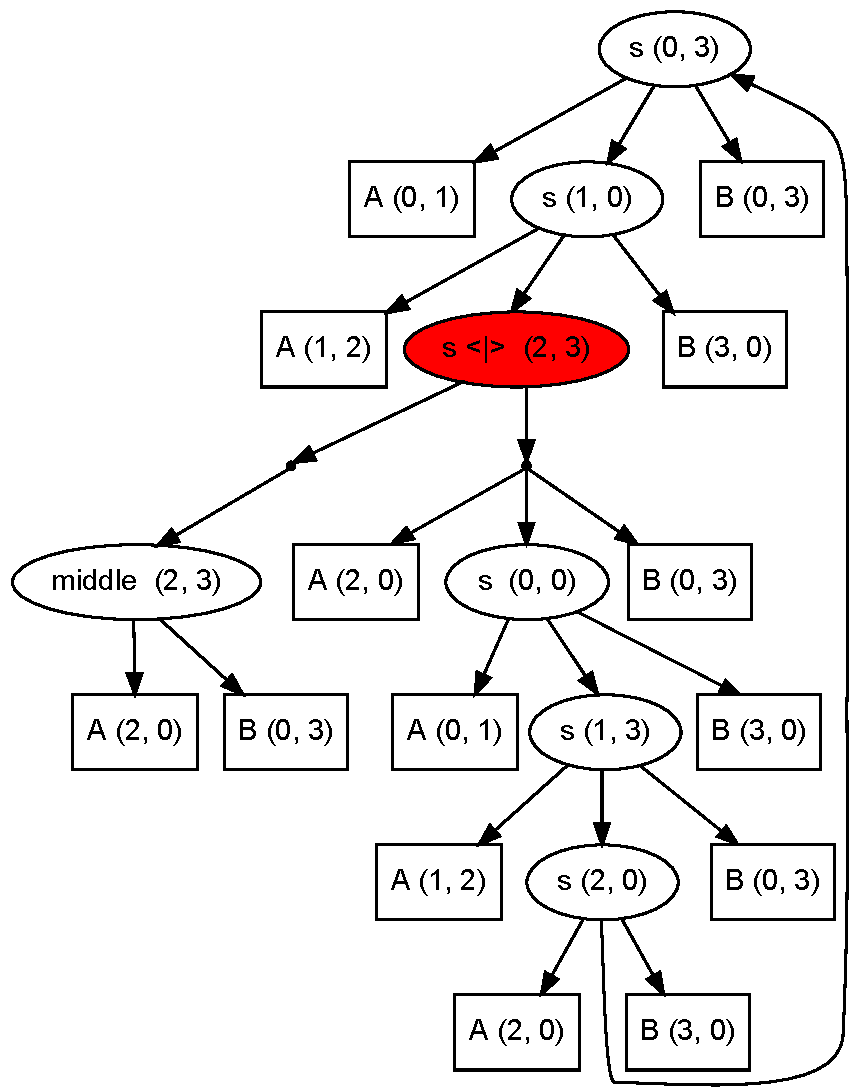
\includegraphics[width=13cm]{dot/AnBn.pdf}
\end{minipage}
}
\\
\begin{minipage}{0.4\textwidth}
    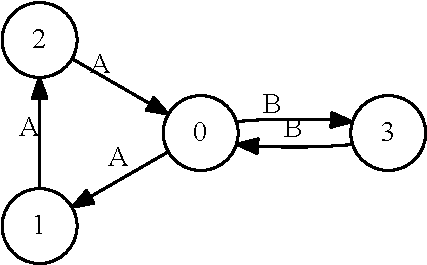
\includegraphics[width=8cm]{dot/input.pdf}
\end{minipage}
\end{tabular}
\end{center}
\end{table}


%% GNUPLOT: LaTeX picture with Postscript
\begingroup
  \makeatletter
  \providecommand\color[2][]{%
    \GenericError{(gnuplot) \space\space\space\@spaces}{%
      Package color not loaded in conjunction with
      terminal option `colourtext'%
    }{See the gnuplot documentation for explanation.%
    }{Either use 'blacktext' in gnuplot or load the package
      color.sty in LaTeX.}%
    \renewcommand\color[2][]{}%
  }%
  \providecommand\includegraphics[2][]{%
    \GenericError{(gnuplot) \space\space\space\@spaces}{%
      Package graphicx or graphics not loaded%
    }{See the gnuplot documentation for explanation.%
    }{The gnuplot epslatex terminal needs graphicx.sty or graphics.sty.}%
    \renewcommand\includegraphics[2][]{}%
  }%
  \providecommand\rotatebox[2]{#2}%
  \@ifundefined{ifGPcolor}{%
    \newif\ifGPcolor
    \GPcolortrue
  }{}%
  \@ifundefined{ifGPblacktext}{%
    \newif\ifGPblacktext
    \GPblacktexttrue
  }{}%
  % define a \g@addto@macro without @ in the name:
  \let\gplgaddtomacro\g@addto@macro
  % define empty templates for all commands taking text:
  \gdef\gplbacktext{}%
  \gdef\gplfronttext{}%
  \makeatother
  \ifGPblacktext
    % no textcolor at all
    \def\colorrgb#1{}%
    \def\colorgray#1{}%
  \else
    % gray or color?
    \ifGPcolor
      \def\colorrgb#1{\color[rgb]{#1}}%
      \def\colorgray#1{\color[gray]{#1}}%
      \expandafter\def\csname LTw\endcsname{\color{white}}%
      \expandafter\def\csname LTb\endcsname{\color{black}}%
      \expandafter\def\csname LTa\endcsname{\color{black}}%
      \expandafter\def\csname LT0\endcsname{\color[rgb]{1,0,0}}%
      \expandafter\def\csname LT1\endcsname{\color[rgb]{0,1,0}}%
      \expandafter\def\csname LT2\endcsname{\color[rgb]{0,0,1}}%
      \expandafter\def\csname LT3\endcsname{\color[rgb]{1,0,1}}%
      \expandafter\def\csname LT4\endcsname{\color[rgb]{0,1,1}}%
      \expandafter\def\csname LT5\endcsname{\color[rgb]{1,1,0}}%
      \expandafter\def\csname LT6\endcsname{\color[rgb]{0,0,0}}%
      \expandafter\def\csname LT7\endcsname{\color[rgb]{1,0.3,0}}%
      \expandafter\def\csname LT8\endcsname{\color[rgb]{0.5,0.5,0.5}}%
    \else
      % gray
      \def\colorrgb#1{\color{black}}%
      \def\colorgray#1{\color[gray]{#1}}%
      \expandafter\def\csname LTw\endcsname{\color{white}}%
      \expandafter\def\csname LTb\endcsname{\color{black}}%
      \expandafter\def\csname LTa\endcsname{\color{black}}%
      \expandafter\def\csname LT0\endcsname{\color{black}}%
      \expandafter\def\csname LT1\endcsname{\color{black}}%
      \expandafter\def\csname LT2\endcsname{\color{black}}%
      \expandafter\def\csname LT3\endcsname{\color{black}}%
      \expandafter\def\csname LT4\endcsname{\color{black}}%
      \expandafter\def\csname LT5\endcsname{\color{black}}%
      \expandafter\def\csname LT6\endcsname{\color{black}}%
      \expandafter\def\csname LT7\endcsname{\color{black}}%
      \expandafter\def\csname LT8\endcsname{\color{black}}%
    \fi
  \fi
    \setlength{\unitlength}{0.0500bp}%
    \ifx\gptboxheight\undefined%
      \newlength{\gptboxheight}%
      \newlength{\gptboxwidth}%
      \newsavebox{\gptboxtext}%
    \fi%
    \setlength{\fboxrule}{0.5pt}%
    \setlength{\fboxsep}{1pt}%
\begin{picture}(5102.00,4534.00)%
    \gplgaddtomacro\gplbacktext{%
      \csname LTb\endcsname%
      \put(1078,704){\makebox(0,0)[r]{\strut{}$0$}}%
      \put(1078,1298){\makebox(0,0)[r]{\strut{}$5000$}}%
      \put(1078,1892){\makebox(0,0)[r]{\strut{}$10000$}}%
      \put(1078,2487){\makebox(0,0)[r]{\strut{}$15000$}}%
      \put(1078,3081){\makebox(0,0)[r]{\strut{}$20000$}}%
      \put(1078,3675){\makebox(0,0)[r]{\strut{}$25000$}}%
      \put(1078,4269){\makebox(0,0)[r]{\strut{}$30000$}}%
      \put(1210,484){\makebox(0,0){\strut{}$0$}}%
      \put(1793,484){\makebox(0,0){\strut{}$10$}}%
      \put(2375,484){\makebox(0,0){\strut{}$20$}}%
      \put(2958,484){\makebox(0,0){\strut{}$30$}}%
      \put(3540,484){\makebox(0,0){\strut{}$40$}}%
      \put(4123,484){\makebox(0,0){\strut{}$50$}}%
      \put(4705,484){\makebox(0,0){\strut{}$60$}}%
    }%
    \gplgaddtomacro\gplfronttext{%
      \csname LTb\endcsname%
      \put(176,2486){\rotatebox{-270}{\makebox(0,0){\strut{}Time in milliseconds}}}%
      \put(2957,154){\makebox(0,0){\strut{}Number of vertices in input graph}}%
      \csname LTb\endcsname%
      \put(1870,4096){\makebox(0,0)[r]{\strut{}$G_0$}}%
      \csname LTb\endcsname%
      \put(1870,3876){\makebox(0,0)[r]{\strut{}$G_2$}}%
      \csname LTb\endcsname%
      \put(1870,3656){\makebox(0,0)[r]{\strut{}$f_1$}}%
      \csname LTb\endcsname%
      \put(1870,3436){\makebox(0,0)[r]{\strut{}$f_2$}}%
    }%
    \gplbacktext
    \put(0,0){\includegraphics{ContextFreeConstrainedPathFindingInGraph-gnuplottex-fig1}}%
    \gplfronttext
  \end{picture}%
\endgroup

%\subsection{Example}

Let us present a solution of task introduced in section~\ref{motivExample}: grammar $G_1$ is a query and we want to find all paths in graph $M$ (presented in picture~\ref{input}) matching this query.
Result SPPF for this input is presented in picture~\ref{SPPF}. Note that presented version does not contains obsolete nodes.
Each terminal node corresponds with edge in the input graph: for each node with label $(v_0, T, v_1)$ there is $e\in E: e=(v_0,T,v_1)$.
We duplicate terminal nodes only for figure simplification.

\begin{figure}[h]
    \begin{center}
        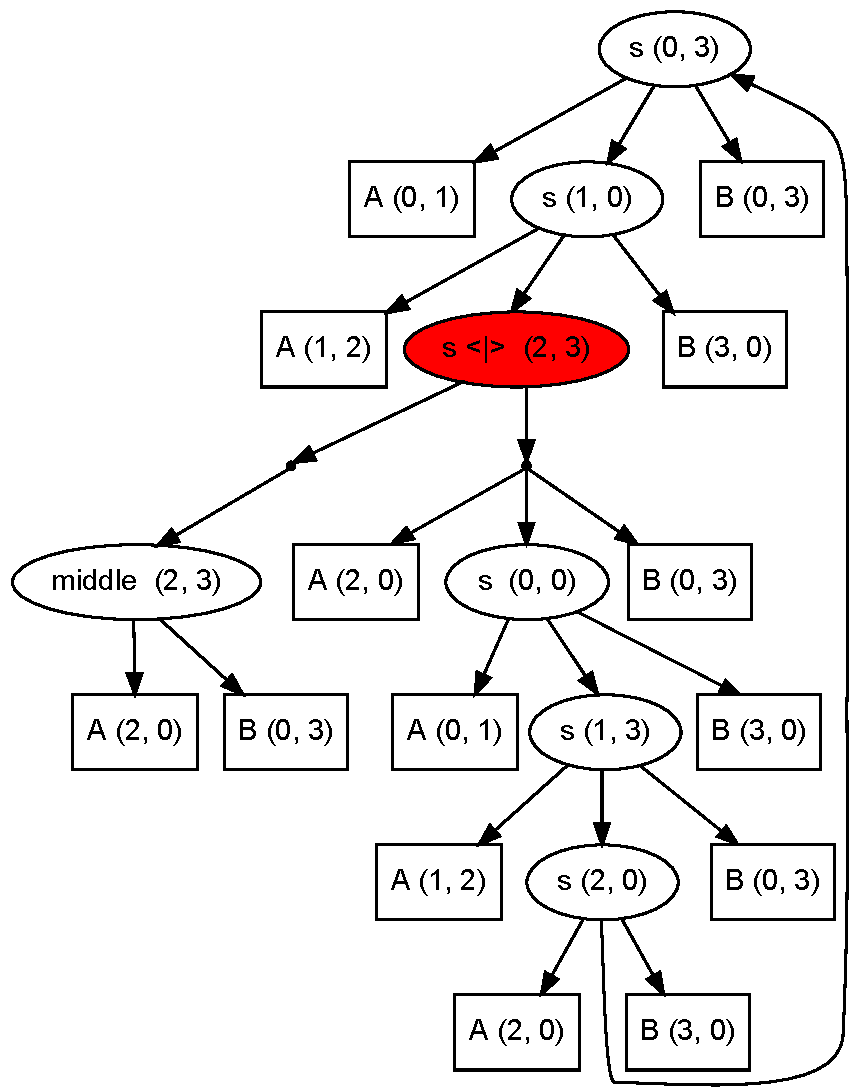
\includegraphics[width=8cm]{dot/AnBn.pdf}
        \caption{Result SPPF for input graph $M$(pic.~\ref{input}) and query $G_1$(pic.~\ref{grammarG})}
        \label{SPPF}        
    \end{center}
\end{figure}

    
As an example of derivation structure usage we can find 'middle' of any path in example above simply by finding correspondent nonterminal $middle$ in SPPF.
So we can find out that there is only one common ancestor for all results, and it is vertex with $id = 0$. 

Extensions stored in nodes allow us to check whether path from $u$ to $v$ exists, and to extract it. 
To extract specified path we need only traverse SPPF, and it can be done in linear time (in terms of SPPF size). 

Lets find paths satisfying specified in $G_1$ constraints from vertex $0$.
To do this we should find vertices with label $(0, s, \_)$ in SPPF.
We can see that there are two vertices with label matched this pattern: $(0, s, 0)$ and $(0, s, 3)$.
At the next step let us to extract corresponded paths from SPPF.
In our example there is cycle in SPPF so there are \textbf{at least} two different paths: $$p_0=\{(0,A,1);(1,A,2);(2,A,0);(0,B,3);(3,B,0);(0,B,3)\}$$ and 
\begin{align*}
p_1=\{&(0,A,1);(1,A,2);(2,A,0);(0,A,1);(1,A,2);(2,A,0);\\ &(0,B,3);(3,B,0);(0,B,3);(3,B,0);(0,B,3);(3,B,0)\}.
\end{align*}


Thus SPPF which was constructed by described algorithm can be useful for query result investigation. 
But in some cases explicit representation of matched subgraph is preferable, and required subgraph that may be extracted from SPPF trivially by its traversal.

%In order to test the resulting solution we have implemented the frontend as a plugin using ReSharper SDK, so it can be installed into ReSharper, Rider and InspectCode.
The source code is parsed by internal ReSharper tools and the result is used to produce graphs and meta-information.
The issues found by the backend are shown using code highlighting.

The first analysis which has been implemented is the considered taint tracking analysis.
It is defined just by the PDA constructed in the section 2 translated into the code with some slight modifications which make it possible to process interactions with object fields.
To provide more information about an issue found by this analysis, the higlighting is accompanied by bulbs containing the full path of tainted variable from the source to the sink represented as the sequence of operations.

\subsection{Sample cases}

Let's look closer at properties of the resulting soluiton.
All these properties are illustrated by screenshots taken exactly from the runned Rider IDE with some small relocations of bulbs to make them not to overlap the code.

Firstly, the solution ensures flow sensitivity. I.e. it processes flow of variables passed into methods and returned from them correctly.
Which can be seen at fig~\ref{fig:ReturnsAndBrackets}.
This example illustrates the most common cases of interprocedural data passing.
\textit{Brackets} method gets the data, performs some computations on them and returns the result.
Invocations at lines 37 and 38 shows that the solution can distinguish two data flow paths despite both of them passes through the same method.
So, \textit{e} becomes tainted because \textit{c} is tainted and \textit{f} does not because \textit{d} is clear.
Moreover, the solution can track paths where passes and returns do not form the correct bracket sequence that is shown by method \textit{PostSource} which does not take any parameter and just returns tainted data.

\begin{figure}[h]
	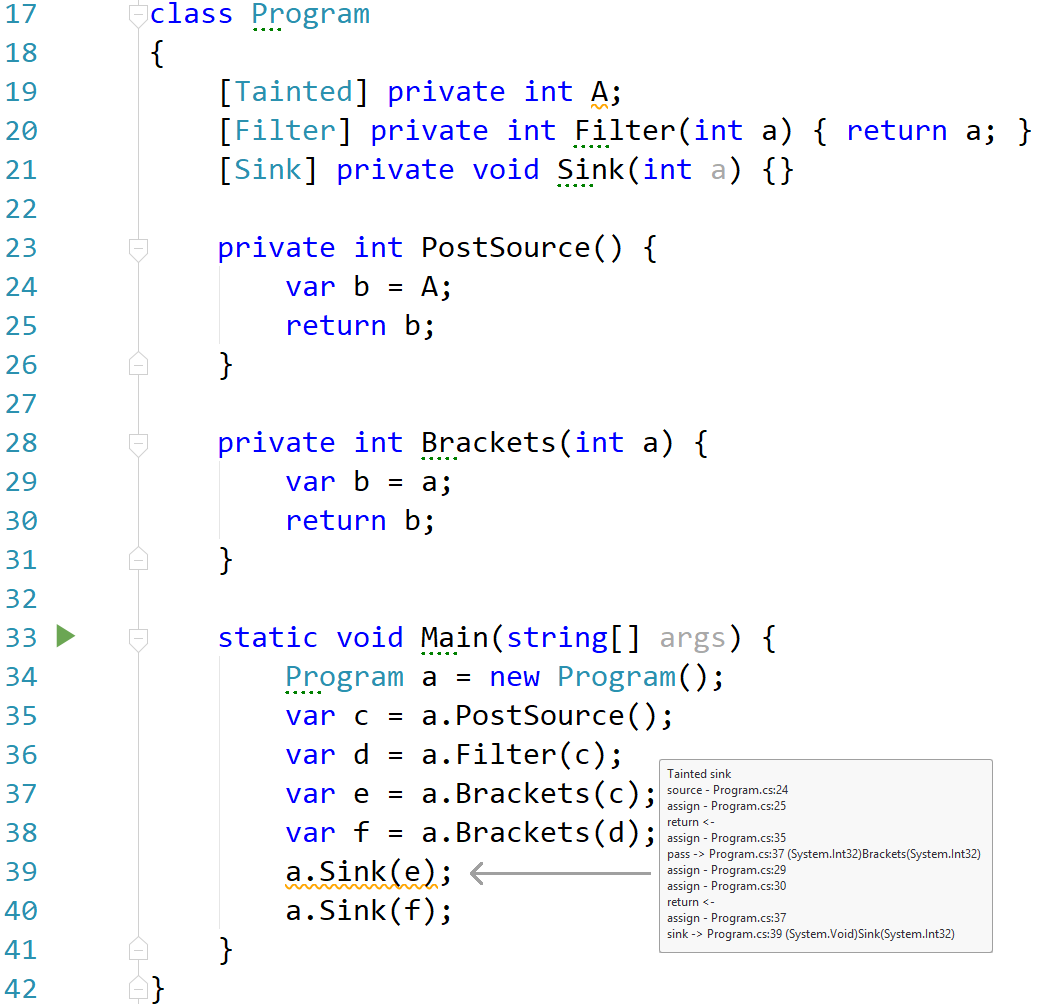
\includegraphics[width=\linewidth]{screenshots/ReturnsAndBrackets.png}
	\caption{Flow sensitivity}
	\label{fig:ReturnsAndBrackets}
\end{figure}

Secondly, the solution has the limited context sensitivity. I.e. it allows to track propagation of objects that are tainted by assigning of some fields inside them both by their own methods and by outer code interacting with their fields directly.
The first case is shown at fig~\ref{fig:ObjectTainting}.
There is the field \textit{B} at the line 18. 
This field can be used widely in the logic of the \textit{Container} class and by this the tainting of this field is considered as the tainting of the whole object.
However, while processing of the method \textit{Store} during the analysis it is hard to decide what the object need to be tainted because in the inner context of \textit{Store} it is just \textit{this} object.
I.e. we must consider the calling context to make such decision.
So, the solution provides this opportunity which is shown by lines 33-36 where the first invocation of \textit{Store} leads to the tainting of object \textit{d} and the second invocation does not taint object \textit{e}.

\begin{figure}[h]
	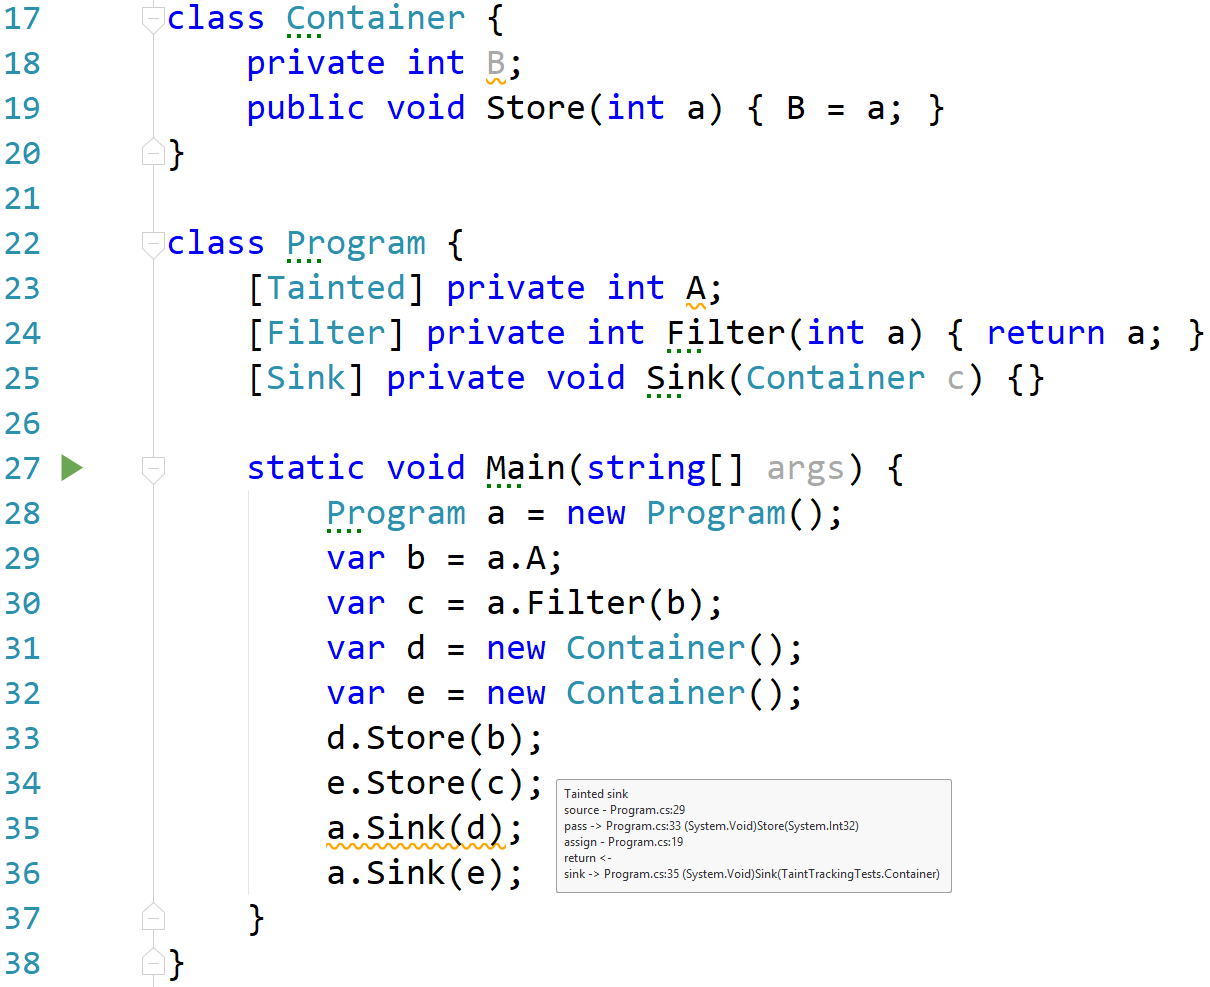
\includegraphics[width=\linewidth]{screenshots/ContextSensitivity.png}
	\caption{Tainting of an object by its own method}
	\label{fig:ObjectTainting}
\end{figure}

Finally, the solution works with any type of recursion and does not fall into infinite cycles.
It can be seen at fig.~\ref{fig:Recursion}.
This snippet contains two mutually recursive methods which pass the data to each other.
The solution checks all possible paths of passing even those which includes cyclic invocations and returns the passed variable to the point corresponding to the initial invocation.

\begin{figure}[h]
	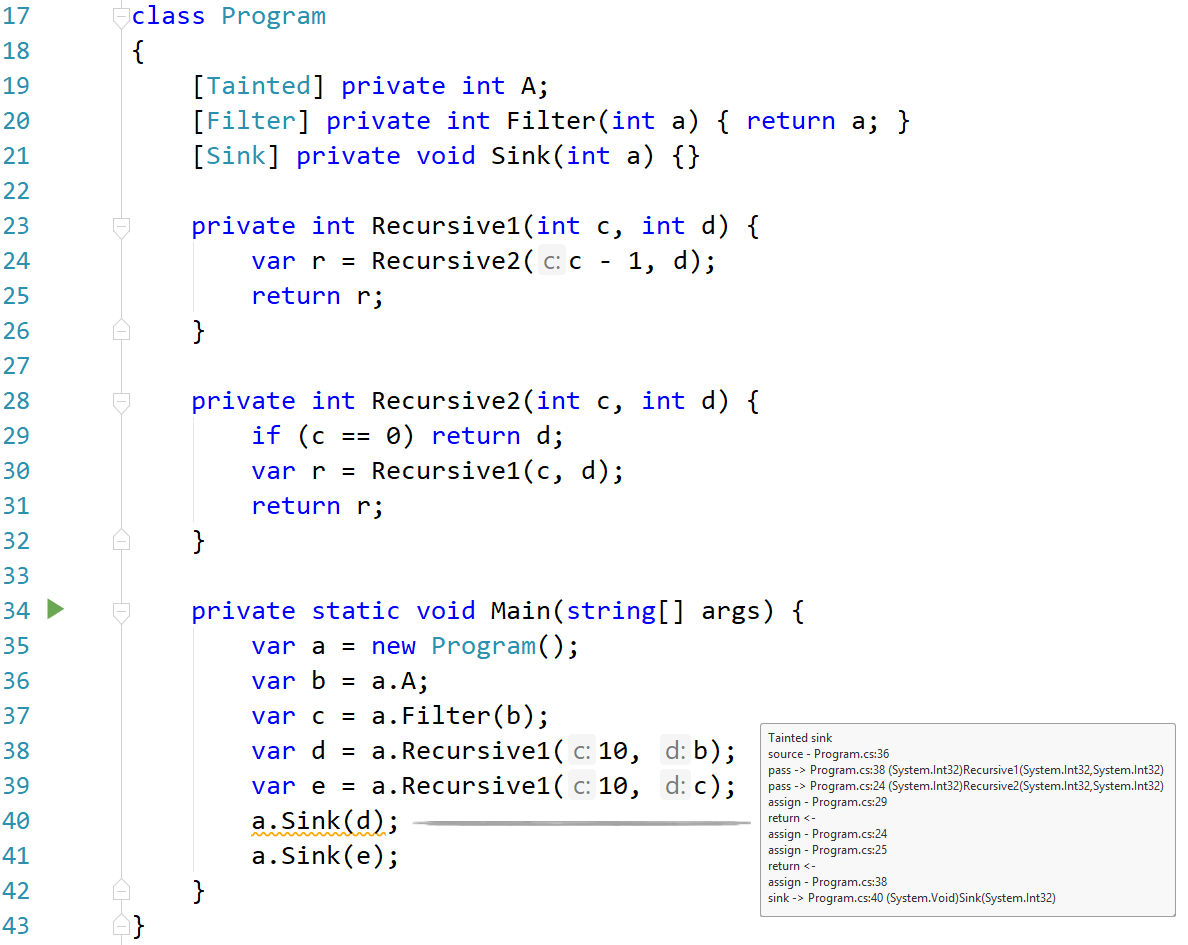
\includegraphics[width=\linewidth]{screenshots/Recursion.png}
	\caption{Recursive methods processing}
	\label{fig:Recursion}
\end{figure}

\subsection{Performance}

It is also necessary to measure the performance of the resulting solution.
Because the implemented taint tracking analysis forces to mark all participating entities manually, it is difficult to perform it on some large project.
However, there is another intermediate analysis which is runned before any other one to collect some information required by resolver.
In particular, it tracks propagation of all variables to discover all possible concrete types of each variable.
So, it involves each variable and each method in the whole program and thus the time and space required for execution of this analysis may be consistent estimation of the efficiency of the solution.

The code base that has been chosen as a source of data is the full solution of the Mono project.
(TODO: ADD SYSTEM CONFIGURATION).
The results is shown in the table~\ref{tab:Performance}.

\begin{table}[h]
	\begin{tabular}{|l|l|l|l|l|}
	\hline
		Project & Classes & Methods & \begin{tabular}[c]{@{}l@{}}Execution \\ time (s)\end{tabular} & \begin{tabular}[c]{@{}l@{}}Allocated \\ memory (GB)\end{tabular} \\ \hline
		Mono & 21013 & 192745 & $21\pm 0.5$ & $\sim 4.2$ \\ \hline
	\end{tabular}
	\caption{Performance}
	\label{tab:Performance}
\end{table}

%\section{Conclusion}

We propose and implement in C\# programming language the generic framework for interprocedural static code analysis implementation.
This framework allows one to implement arbitrary interprocedural analysis in terms of CFL-reachability.
By using the proposed framework, we implement a plugin upon ReSharper infrastructure which provides simple taint analysis and demonstrate that our solution can handle important real-world cases.
Also we show that the proposed framework can be used for real-world solutions analysis.

One of the directions for future work is a creation of analysis and its evaluation on real-world projects.
By this way, we want to get information which helps to improve the usability of our framework: tune performance, improve API, etc.
Also we should improve documentation and create more examples of usage.

Another direction is a practical evaluation of automatic fix location prediction by using minimum cuts method~\cite{10.1007/978-3-319-63390-9_27}.

Also we want to compare the proposed approach with other generic CFL-reachability based approaches for interprocedural code analysis cretion. For example, fith generation-based approach~\cite{LPAR-21:Cauliflower_Solver_Generator_for}, which idea is similar to parser generators.


%\bibliographystyle{abbrv}
%\bibliography{ContextFreeConstrainedPathFindingInGraph}
%\end{landscape}
\end{document}
